\documentclass[hidelinks,11pt,dvipsnames]{article}
% xcolor commonly causes option clashes, this fixes that
\PassOptionsToPackage{dvipsnames,table}{xcolor}
\usepackage[tmargin=1in, bmargin=1in, lmargin=0.8in, rmargin=1in]{geometry}

%%%%%%%%%%%%%%%%%%%%%%%%%%%%%%%%%%%%%%%%%%%%%%%%%%%%%%%%%%%%%%%%%%%%
%%% For inkscape-figures
%%% Assumes the following directory structure:
%%% master.tex
%%% figures/
%%%     figure1.pdf_tex
%%%     figure1.svg
%%%     figure1.pdf
%%%%%%%%%%%%%%%%%%%%%%%%%%%%%%%%%%%%%%%%%%%%%%%%%%%%%%%%%%%%%%%%%%%%
%\usepackage{import}
\usepackage{pdfpages}
\usepackage{transparent}

\newcommand{\incfig}[2][1]{%
    \def\svgwidth{#1\columnwidth}
    \import{./figures/}{#2.pdf_tex}
}

\pdfsuppresswarningpagegroup=1

% enable synctex for inverse search, whatever synctex is
\synctex=1
\usepackage{float,macrosabound,homework,theorem-env}
\usepackage{microtype}


% font stuff
\usepackage{sectsty}
\allsectionsfont{\sffamily}
\linespread{1.1}

% bibtex stuff
\usepackage[backend=biber,style=alphabetic,sorting=anyt]{biblatex}
\addbibresource{main.bib}

% colored text shortcuts
\newcommand{\blue}[1]{\color{MidnightBlue}{#1}}
\newcommand{\red}[1]{\textcolor{Mahogany}{#1}}
\newcommand{\green}[1]{\textcolor{ForestGreen}{#1}}


% use mathptmx pkg while using default mathcal font
\DeclareMathAlphabet{\mathcal}{OMS}{cmsy}{m}{n}

% fixes the positioning of subscripts in $$ $$
\renewcommand{\det}{\operatorname{det}}

\usetikzlibrary{positioning, arrows.meta}
\newcommand{\here}[2]{\tikz[remember picture]{\node[inner sep=0](#2){#1}}}

%%%%%%%%%%%%%%%%%%%%%%%%%%%%%%%%%%%%%%%%%%%%%%%%%%%%%%%%%%%%%%%%%%%%%
%%% Entry Counter
%%%%%%%%%%%%%%%%%%%%%%%%%%%%%%%%%%%%%%%%%%%%%%%%%%%%%%%%%%%%%%%%%%%%%
\newcounter{entry-counter}
\newcommand{\entry}[1]
{
	\addtocounter{entry-counter}{1}
    \tchap{Entry \arabic{entry-counter}}
	%\addcontentsline{toc}{section}{Entry \arabic{entry-counter}: #1}
	\vspace{-1.5em}
    \begin{center}
		\small \emph{Written: #1}
    \end{center}
}

\usepackage{titling}
\renewcommand\maketitlehooka{\null\mbox{}\vfill}
\renewcommand\maketitlehookd{\vfill\null}


\usepackage{capt-of}
\usepackage{tikz}
\usepackage{listings}
\usetikzlibrary{positioning,calc,intersections,through,backgrounds, shapes.geometric, decorations.markings,arrows}

\def\sset{\subseteq}
\def\iso{\cong}
\def\gend#1{\langle #1\rangle}

\newcommand{\rightoverleftarrow}{%
  \mathrel{\vcenter{\mathsurround0pt
    \ialign{##\crcr
      \noalign{\nointerlineskip}$\longrightarrow$\crcr
      \noalign{\nointerlineskip}$\longleftarrow$\crcr
    }%
  }}%
}

\newcommand\makesphere{} % just for safety
\def\makesphere(#1)(#2)[#3][#4]{%
  % Synopsis
  % \makesphere[draw options](center)(initial angle:final angle:radius)
  \shade[ball color = #3, opacity = #4] #1 circle (#2);
  \draw #1 circle (#2);
  \draw ($#1 - (#2, 0)$) arc (180:360:#2 and 3*#2/10);
  \draw[dashed] ($#1 + (#2, 0)$) arc (0:180:#2 and 3*#2/10);
}
% same thing as makesphere but places white background behind
\newcommand\altmakesphere{} % just for safety
\def\altmakesphere(#1)(#2)(#3)[#4][#5]{%
  % Synopsis
  % \make sphere[draw options](center)(initial angle:final angle:radius)
  \draw [fill=white!30] #1 circle (#2);
  \shade[ball color = #4, opacity = #5] #1 circle (#2);
  \draw #1 circle (#2);
  \draw ($#1 - (#2, 0)$) arc (180:360:#2 and 3*#2/10);
  \draw[dashed] ($#1 + (#2, 0)$) arc (0:180:#2 and 3*#2/10);
  \node at #1 {#3};
}

\begin{document}
% set section number to 1
% fixes theorem numbering without need to have a section title
\setcounter{section}{1}

\pagestyle{empty}
	\LARGE
\begin{center}
	Foundations of Data Science and Machine Learning -- \emph{Homework 3}\\
	\Large
	Isaac Martin \\
    Last compiled \today
\end{center}
\normalsize
\vspace{-4mm}
\hru

\begin{homework}[e]
  \prob[\textsc{Exercise 1.}] (Completed this one last, too lazy to copy down the problem statement.)
  \begin{soln}
    There isn't a lot to say in this problem, it is mostly implementation and experimentation. We discuss our process and our results. The code is attached to the end of this document. Throughout this problem a kmeans++ initialization was used with 10 iterations.
    \begin{enumerate}[(a)]
      \item We first generate a matrix $C$ (named ``$X$'' in the code) as the requested block matrix. We then create the random matrix $A$ by drawing from a Bernoulli distribution at each entry, using the entry's value of 0.3 or 0.7 as the probability in the Bernoulli distribution. Finally, we generate a random permutation matrix $P$ and conjugate $A$ by $P$. We save the inverse of $P$ for use later in ``unshuffling'' the labels generated by kmeans in each case.

        We then use scikit-learn's implementation of kmeans to cluster the rows of $A$ and store both the cost of the final clustering and the cluster labels for each row. By applying the inverse permutation to the list of labels, we can easily compare it to the natural permutation in the problem statement. Here is the unshuffled list of labels:

        \begin{center}
          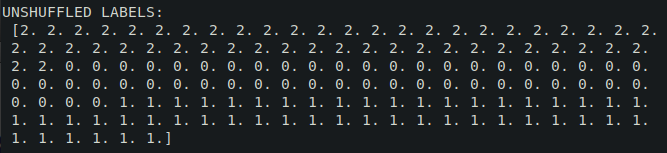
\includegraphics[width=12cm]{~/Desktop/university/latex/phd/data-sci/figures/hwk3-prob1a.png}
          \captionof{figure}{List of labels generated by kmeans}
          \label{fig:prob1a}
        \end{center}
        It should resemble a list which looks like $[0,0,...,0,1,1,...,1,2,2,....,2]$, and indeed it does, up to rearranging the $0$'s, $1$'s and $2$'s. Note that the index on the cluster is arbitrary, so this rearrangement is to be expected.
        \item We now apply the kmeans algorithm as done in part (a) for many different values of $k$ and plot the costs in each case. People have noticed that the resulting graph often looks like an elbow -- the cost drops tremendously at a certain choice of $k$, after which the addition of extra clusters only incrementally improves the cost of the obtained clustering. This is precisely what we observe here. The ``elbow'' point occurs at $k = 3$, meaning this is a good choice for the number of clusters.

        \begin{center}
          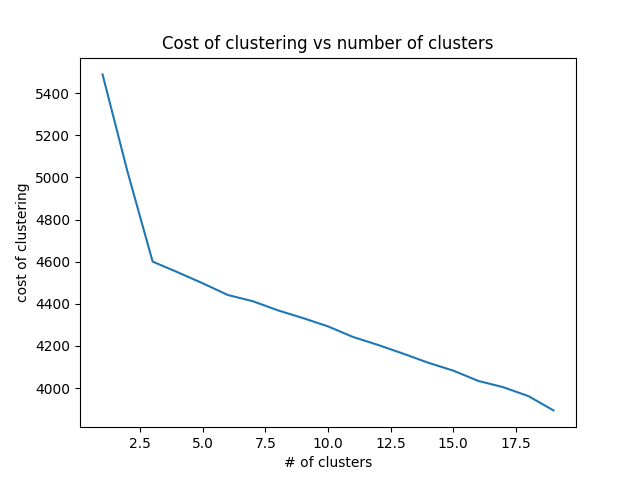
\includegraphics[width=12cm]{~/Desktop/university/latex/phd/data-sci/figures/hwk3-figure1.png}
          \captionof{figure}{List of labels generated by kmeans}
          \label{fig:prob1b}
        \end{center}

      \item We now apply the same procedure as in part (a), but this time we redefine $A = A\Phi$ where $\Phi$ is a $150 \times 10$ spherically sampled Gaussian matrix. We recover something resembling the original clustering, but it isn't great; we observe many rows have randomly jumped clusters.
        \begin{center}
          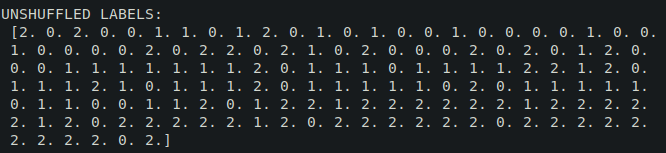
\includegraphics[width=12cm]{~/Desktop/university/latex/phd/data-sci/figures/hwk3-prob1c.png}
          \captionof{figure}{List of labels generated by kmeans in problem 1 (c). Some of the natural clustering has been recovered, but it is far from a good match.}
          \label{fig:prob1c}
        \end{center}
        This suggests that the Gaussian projection isn't a great way to preserve the clustering structure of our original data.
      \item We now apply a projection to $\bR^3$ using the first three right singular vectors of $A$. This proves to be a much better way to preserve the clustering structure of $A$; for while there is still some differences, it recovers the original clustering much better than the Gaussian projection. Problem 2 (b) explains this.
        \begin{center}
          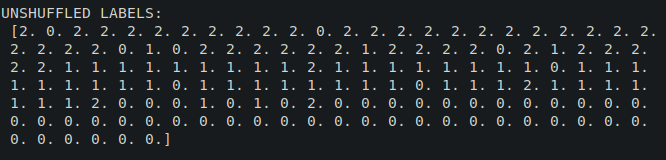
\includegraphics[width=12cm]{~/Desktop/university/latex/phd/data-sci/figures/hwk3-prob1d.png}
          \captionof{figure}{List of labels generated by kmeans in problem 1 (d). Most of the original clustering has been recovered, despite the fact that we have reduced from $150$ dimensions to $3$.}
          \label{fig:prob1d}
        \end{center}
    \end{enumerate}
  \end{soln}
  \prob[\textsc{Exercise 2.}] Let $\bfX\in \bR^{n\times d}$ be a matrix whose $n$ rows are the data points $\bfx_1,...,\bfx_n \in \bR^d$, and let $\cX = \{\bfx_1,...,\bfx_n\}$. Consider the $k$-means optimization problem: find a partition $C_1,...,C_k$ which minimizes, among all partitions of $[n]$ into $k$ subsets,
  \begin{align*}
    \operatorname{cost}_{\cX}(C_1,...,C_k):= \sum_{j=1}^k\sum_{i \in C_j} \left\|\bfx_i - \frac{1}{|C_j|}\sum_{i\in C_j} \bfx_i\right\|^2_2.
  \end{align*}
  \begin{enumerate}[(a)]
    \item Suppose that $\Phi:\bR^d \to \bR^r$ with $r = \cO(\log(n)/\epsilon^2)$ is a random i.i.d. spherical Gaussian projection matrix and thus satisfies the JL lemma. Consider the projected points $\bfy_j = \Phi\bfx_j\in \bR^r$ and suppose $\tilC_1,...,\tilC_k$ are an optimal set of $k$-means clusters for the data points $\cY = \{\bfy_1,....,\bfy_n\}$. That is,
    \begin{align*}
      \operatorname{cost}_{\cY}(\tilC_1,...,\tilC_n) = \min_{C_\bullet}\cost_{\cY}(C_1,...,C_k)
    \end{align*}
    where the minimization is over all partitions of $\cY$ into $k$ subsets. Show that the clusters $\tilC_1,...,\tilC_k$ also represent a good clustering for the original dataset $\cX$ in the sense that with high probability
    \begin{align*}
      \cost_\cX(\tilC_1,...,\tilC_k) \leq (1 + \epsilon)\min_{C_1,...,C_k}\cost_\cX(C_1,...,C_k).
    \end{align*}

  \item Suppose we now project the points $\bfx_j$ to $k$ dimensions using the SVD of $\bfX$. Let $\bfV_k\in \bR^{d\times k}$ be the matrix whose columns are the first right singular vectors of $\bfX$. Suppose the $\tilC_1,...,\tilC_k$ are the optimal $k$-means clusters for the points $\bfV_k^\top\bfx_1,...,\bfV_k^\top\bfx_n$.

    Show that the clusters $\bfC_1,...,\bfC_k$ also represent a good clustering for the original dataset $\cX$, in the sense that
    \begin{align*}
      \cost_\cX(\tilC_1,...,\tilC_k)) \leq 2 \min_{C_1,...,C_k} \cost_{\cX}(C_1,...,C_k).
    \end{align*}
  \end{enumerate}
  \begin{prf}$ $
    \begin{enumerate}[(a)]
      \item First consider a fixed $j \in \{1,...,k\}$ and the following expression:
        \begin{align*}
          \sum_{i,\ell\in C_j} \|\bfx_i - \bfx_j\|^2_2 = \sum_{i\in C_j}\sum_{\ell \in C_j} \|\bfx_i - \bfx_j\|^2_2.
        \end{align*}
        Letting $\mu_j = \frac{1}{|C_j|}\sum_{i \in C_j}\bfx_i$ denote the centroid of $\{\bfx_i\}_{i \in C_j}$, we see that
        \begin{align*}
          \sum_{i\in C_j}\sum_{\ell \in C_j} &\|\bfx_i - \bfx_j\|^2_2 
            =\sum_{i\in C_j}\sum_{\ell \in C_j} \|\bfx_i - \mu_j + \mu_j - \bfx_j\|^2_2 \\
            &= \sum_{i\in C_j}\left(\sum_{\ell \in C_j}\|\mu_j - \bfx_\ell\|^2_2 ~+~ 2(\bfx_i - \mu_j)\cdot\sum_{\ell \in C_j}(\mu_j - \bfx_\ell) ~+~ |C_j|\cdot \|\bfx_i - \mu_j\|^2_2\right).
        \end{align*}
        The second equality above follows from the fact that
        \begin{align*}
          \sum_{i=1}^n \|\bfa_i - \bfc + \bfc - \bfx\|^2 = \sum_{i=1}^n \|\bfa_i - \bfc\| ~+~ 2(\bfc - \bfx) \cdot \sum_i (\bfa_i - \bfc) ~+~ n\cdot\|\bfc - \bfx\|^2,
        \end{align*}
        which in turn can be derived by writing $\|\bfa_i - \bfc + \bfc - \bfx\|^2 = \langle \bfa_i - \bfc + \bfc - \bfx, \bfa_i - \bfc + \bfc - \bfx\rangle$, expanding by bilinearity and gathering up terms in a clever way. Using the fact that indexing over $\ell$ and $i$ is equivalent together with the bilinearity properties of the inner product, we can continue our above chain of equalities to get that
        \begin{align*}
          \sum_{i,\ell\in C_j} &\|\bfx_i - \bfx_j\|^2_2  \\
            &= \sum_{i\in C_j}\left(\sum_{\ell \in C_j}\|\mu_j - \bfx_\ell\|^2_2 ~+~ 2(\bfx_i - \mu_j)\cdot\sum_{\ell \in C_j}(\mu_j - \bfx_\ell) ~+~ |C_j|\cdot \|\bfx_i - \mu_j\|^2_2\right) \\
            &= |C_j|\cdot \sum_{\ell\in C_j} ~+~ 2\left(\sum_{\ell \in C_j}(\mu_j - \bfx_\ell)\right)\cdot \sum_{i\in C_j}(\bfx_i - \mu_j) ~+~ |C_j|\cdot\sum_{i\in C_j} \|\bfx_i - \mu_j\|^2_2 \\
            &= 2|C_j|\cdot \sum_{i\in C_j} \|\bfx_i - \mu_j\|^2_2 ~-~ 2 \left\|\sum_{\ell \in C_j}(\bfx_i - \mu_j)\right\|^2_2.
        \end{align*}
        The term $\sum_{\ell \in C_j}(\bfx_i - \mu_j)$ is $0$ because $\mu_j$ is the centroid of $\{\bfx_i\}_{i\in C_j}$, hence
        \begin{align*}
          \sum_{i,\ell\in C_j} &\|\bfx_i - \bfx_j\|^2_2 
          = 2|C_j|\cdot \sum_{i\in C_j} \|\bfx_i - \mu_j \|^2_2 = 2|C_j|\cdot \sum_{i\in C_j} \left\|\bfx_i -  \frac{1}{|C_j|}\sum_{\ell \in C_j}\bfx_\ell\right\|^2_2.
        \end{align*}
        Taking sums over all $j \in \{1,...,k\}$, we then get that
        \begin{align*}
          \cost_\cX(C_1,...,C_k) &= \sum_{j=1}^k\sum_{i \in C_j} \left\|\bfx_i - \frac{1}{|C_j|}\sum_{i\in C_j} \bfx_i\right\|^2_2 \\
                                  &= \sum_{j=1}^k \frac{1}{2|C_j|}\sum_{i,\ell \in C_j}\|\bfx_i - \bfx_\ell\|^2_2,
        \end{align*}
        as suggested by the hint. This form of the cost function integrates more favorably with the properties of the Johnson-Lindenstrauss theorem, since for $r > C\cdot \frac{\log(n/\delta)}{\epsilon^2}$, we get that
        \begin{align*}
          \left\|\bfy_i - \bfy_j\right\|^2_2  = \|\Phi(\bfx_i - \bfx_\ell)\|^2_2 \leq (1 + \epsilon)\|\bfx_i - \bfx_\ell\|^2_2
        \end{align*}
        occurs with probability at least $1 - \delta$ and therefore
        \begin{align*}
          \cost_\cY(C_1,...,C_k) &= \sum_{j=1}^k\frac{1}{2|C_j|}\sum_{i,\ell\in C_j} \|\bfy_i - \bfy_\ell\|^2_2 \\
          &\leq (1 + \epsilon)\sum_{j=1}^k\frac{1}{2|C_j|}\sum_{i,\ell\in C_j} \|\bfx_i - \bfx_\ell\|^2_2 = (1+\epsilon)\cost_\cX(C_1,...,C_k)
        \end{align*}
        also occurs with probability at least $1 - \delta$ for any partition $C_1 \sqcup ... \sqcup C_k = \{1..n\}$. Combining this with the other bound from the JL theorem we have that
        \begin{align*}
          (1-\epsilon)\cost_\cX(C_1,...,C)k \leq \cost_\cY(C_1,...,C_k) \leq (1+\epsilon)\cost_\cX(C_1,...,C_k)
        \end{align*}
        for all partitions $C_\bullet$ of $\cX$. Since this holds for all partitions of $\cX$ it also holds for the partition $\tilC_\bullet$ which minimizes $\cost_\cY$, hence
        \begin{align*}
          (1 - \epsilon)\cost_\cX(\tilC_1,...,\tilC_k) \leq \cost_\cY(\tilC_1,...,\tilC_k) \leq \cost_\cY(C_1,...,C_k) \leq (1+\epsilon)\cost_\cX(C_1,...,C_k).
        \end{align*}
        We then have that
        \begin{align*}
          \cost_\cX(\tilC_1,...,\tilC_k) \leq \frac{1+\epsilon}{1-\epsilon}\cost_\cY(C_1,...,C_k).
        \end{align*}
        This is not quite what we want. However, we chose $r = \cO(\log(n)/\epsilon^2)$, which only means that $r = C\log(n)/\epsilon^2$ for some $C$. Rescale $C$ and choose a new $\epsilon' \in (0,1)$ so that
        \begin{align*}
          r = 9C\cdot \frac{\log(n)}{\epsilon'^2} \implies \epsilon = 3\sqrt{\frac{C\log(n)}{r}} = 3 \epsilon.
        \end{align*}
        If our original $\epsilon$ was less than $1/3$, then
        \begin{align*}
          1 - 3\epsilon > 0 
            &\iff 0 < \epsilon(1 - 3\epsilon) \\
            &\iff  1 + \epsilon < 1 + 3\epsilon - \epsilon - 3\epsilon^2\\
            &\iff \frac{1+\epsilon}{1 - \epsilon} < 1 + 3\epsilon = 1 + \epsilon'.
        \end{align*}
        Thus, for $\epsilon'$, we have
        \begin{align*}
          \cost_\cX(\tilC_1,...,\tilC_k) \leq \frac{1+\epsilon}{1-\epsilon}\cost_\cY(C_1,...,C_k) \leq (1+\epsilon')\cost_\cY(C_1,...,C_k).
        \end{align*}
        This is perfectly fine, since the change $\epsilon \to \epsilon'$ corresponds to scaling $r$ by $r$, and hence we still have that $r = \cO(\log(n)/\epsilon^2)$ for our original choice of $\epsilon$. This gives us the desired result.

    \item We first prove that $\cost_\cX(C_1,...,C_k) = \|\bfX - MM^\top\bfX\|^2_F$ where $M\in \bR^{n\times k}$is defined by $M_{ij} = \frac{1}{\sqrt{|C_j|}}$ if $i \in C_j$ and $0$ otherwise. Notice that each row of $M$ has only one nonzero element at index $(i,j)$ where $i \in C_j$, and hence
      \begin{align*}
        [MM^\top]_{ij} = [M]_{i,\bullet} \cdot [M]_{j,\bullet} =
        \begin{cases}
          \frac{1}{|C_{\ell_i}} & i,j \in C_{\ell_i} \\
          0 & \text{else}
        \end{cases}
      \end{align*}
      for some $\ell_i = 1,...,k$. In particular, each diagonal element $[MM^\top]_{ii}$ is nonzero and is equal to $1/|C_{\ell_i}|$ where $i \in C_{\ell_i}$. Thus, when we multiply a row $[MM^\top]_{i,\bullet}$ by a column $[\bfX]_{\bullet,j}$ of $\bfX$, the result is a sum
      \begin{align*}
        [MM^\top\bfX]_{ij} = \frac{1}{|C_{\ell_i}}\sum_{a \in C_{\ell_i}} \bfx_{a}^j
      \end{align*}
      where $C_{\ell_i}$ is the partition containing $i$ and $\bfx_a^j$ is the $j$th term in the data point $\bfx_a$. That is, $[MM^\top\bfX]_{ij}$ is the sum of the $j$th components of all data points belonging to $C_{\ell_i}$ scaled by $1/|C_{\ell_i}|$. The $i$th row of $MM^T\bfX$ is therefore the centroid of the $\ell_i$th cluster $\{\bfx_j\}_{j \in C_{\ell_i}}$. Denoting by $\mu_{\ell_i}$ the $\ell_i$th centroid, we see that
      \begin{align*}
        \|\bfX - MM^\top\bfX\|^2_F 
          &= \sum_{i=1}^n\|[\bfX - MM^\top\bfX]_{i,\bullet}\|^2 \\
          &= \sum_{i=1}^n\|\bfx_i - \mu_{\ell_i}\|^2 \\
          &= \sum_{j=1}^k\sum_{i\in C_j} \|\bfx_i - \mu_i\|^2 = \cost_\cX(C_1,...,C_k).
      \end{align*}
      This gives us yet another expression for the $k$-means cost function.

      We now turn to the problem in earnest. Let $\{v_1,...,v_k,v_{k+1},...,v_d\}$ be the complete list of right singular vectors for $X$, and note that they form a complete orthonormal basis for $\bR^d$. Here we use the formulation of SVD in which $V$ and $U$ are both orthogonal matrices (not $d\times r$ matrices) but whose smallest singular vectors might correspond to singular values of 0. Let $W$ be the matrix whose columns are $v_{k+1},...,v_d$. Then $V = V_k\oplus W$ is a $d\times d$ orthogonal matrix, preserves the Frobenius norm, and hence
      \begin{align*}
        \cost_\cX(\tilC_1,...,\tilC_k) 
          &= \|\bfX - \tilM\tilM^\top\bfX\|^2_2 = \|(\bfX - \tilM\tilM^\top\bfX)(V_k\oplus W)\|^2_2 \\
          &= \|(\bfX V_k - \tilM\tilM^\top\bfX V_k) \oplus (\bfX W - \tilM\tilM^\top\bfX W)\|^2_2 \\
          &= \|(\bfX V_k - \tilM\tilM^\top\bfX V_k)\|^2_2 + \|(\bfX W - \tilM\tilM^\top \bfX W)\|^2_2
      \end{align*}
      where $\tilM$ is the matrix defined earlier corresponding to the clustering $\tilC_\bullet$. If we can bound both of these summands by $\cost_\cX(C_1,...,C_k)$ for an arbitrary clustering $C_\bullet$, then we will be done. Let $M$ denote the matrix corresponding to this $C_\bullet$.

      The first term is easy. Note first that $\tilC_\bullet$ is an optimal choice of clustering for $\bfX V_k$, and hence
      \begin{align*}
         \|(\bfX V_k - \tilM\tilM^\top\bfX V_k)\|^2_2 = \cost_\cY(\tilC_\bullet)\leq \cost_\cY(C_\bullet) = \|(\bfX V_k - MM^\top\bfX V_k)\|^2_2.
      \end{align*}
      However, by what we have above,
      \begin{align*}
        \|(\bfX V_k - MM^\top\bfX V_k)\|^2_2 \leq \|(\bfX V_k - MM^\top\bfX V_k)\|^2_2 + \|(\bfX W - MM^\top\bfX W)\|^2_2 = \cost_\cX(C_\bullet),
      \end{align*}
      so we have that $\cost_\cY(\tilC_\bullet) \leq \cost_\cX(C_\bullet)$.
    \end{enumerate}

    The next term is much harder. The first thing we must note is that the matrix $I_n - MM^\top$ has operator norm 1. This can be seen via direct computation by looking at its action on an arbitrary norm 1 vector. There truly ought to be a better way to see this -- I worked this out on paper but do not entirely trust my result, and hence don't include it here.

    However, if we take $\|I_n - MM^\top\|_2 \leq 1$ as a given, then we see that
    \begin{align*}
      \|\bfX W - MM^\top\bfX W\|^2_F = \|(I_n - MM^\top)\bfX W\|^2_F \leq \|\bfX W\|^2_F.
    \end{align*}
    This last equality follows from the definition of the operator norm -- for each column $c_i$ in $\bfX W$, $\|(I_n - MM^\top)c_i\| \leq \|c_i\|$, and hence
    \begin{align*}
      \|(I_n - MM^\top)\bfX W\| \leq \|c_1\|^2 + ... + \|c_d\|^2 = \|\bfX W\|^2_F.
    \end{align*}
    The matrix $\bfX W$ is interesting. Writing $X = U\Sigma V^\top$, we see that by the normalicy of the right singular vectors
    \begin{align*}
      X W = U\Sigma V^\top W = U \Sigma \cdot 
      \begin{pmatrix}
        0 & \vline & 0 \\
        \hline
        0 & \vline & I_{d - k}
      \end{pmatrix} = U\cdot 
      \begin{pmatrix}
        0 & \vline & 0 \\
        \hline
        0 & \vline & \Sigma - \Sigma_k
      \end{pmatrix},
    \end{align*}
    meaning that $XW$ is the result of taking the product of $U$ together with the diagonal matrix consisting of only the final $d - k$ singular values. By the previous homework, we then get that
    \begin{align*}
      \|\bfX W\|^2_F = \sigma_{k+1}^2 + ... + \sigma_d^2 = \|\bfX - \bfX_k\|^2_F.
    \end{align*}
    This is something we can work with. By the hint, $MM^\top\bfX$ has rank $k$, but we have seen that $X_k$ minimizes $\|X - C\|^2_F$ among rank $k$ matrices, hence
    \begin{align*}
      \|(\bfX W - \tilM\tilM^\top \bfX W)\|^2_2 \leq \|\bfX W\|^2_F = \|X - X_k\|^2_F \leq \|\bfX - MM^\top \bfX\|^2_F.
    \end{align*}
    This is the desired bound. Putting this all together, we get that
    \begin{align*}
      \cost_\cX(\tilC_\bullet)
          &= \|(\bfX V_k - \tilM\tilM^\top\bfX V_k)\|^2_2 + \|(\bfX W - \tilM\tilM^\top \bfX W)\|^2_2 \\
          &\leq \cost_\cX(C_\bullet) + \cost_\cX(C_\bullet) = 2\cost_\cX(C_\bullet).
    \end{align*}
    Since this holds for all partitions $C_\bullet$, it holds for the one which minimizes $\cost_\cX(C_\bullet)$ as well, and so we have our result.
  \end{prf}
  \prob[\textsc{Exercise 3.}] Find the mapping $\varphi(\bfx)$ that gives rise to the polynomial kernel \begin{align*}
    K(\bfx, \bfy) = (x_1x_2 + y_1y_2)^2.
  \end{align*}
  \begin{prf}
    Consider the map $\varphi:\bR^2 \to \bR^3$ defined $\varphi(x_1,x_2) = (x_1^2, x_2^2, \sqrt{2}x_1x_2)$. Interestingly, this is similar to the map one considers from a polynomial ring $R[x_1,x_2]$ to its $2^{\text{nd}}$ Veronese subring $R[x_1^2,x_1x_2,x_2^2]$. We then have that
    \begin{align*}
      \varphi(\bfx)\cdot \varphi(\bfy)^T
        &= (x_1^2,x_2^2,\sqrt{2}x_1x_2) \cdot (y_1^2,y_2^2, \sqrt{2}y_1y_2) \\
        &= x_1^2y_1^2 + x_2^2y_2^2 + 2x_1y_1x_2y_2 \\
        &= (x_1y_1 + x_2y_2)^2,
    \end{align*}
    hence $\varphi$ gives rise to the desired kernel.
  \end{prf}
  \prob[\textsc{Exercise 4.}] Consider a Support Vector Machine with ``soft margin'' constrains which allows for misclassification: Given training data $(\bfx_1,y_1),...,(\bfx_n,y_n)$ where $\bfx_j \in \bR^d$ and $y_j \in \{-1, +1\}$, the SVM is
  \begin{align*}
    \min_{\bfw, b,\xi} ~ \lambda\|\bfw\|^2_2 + \frac{1}{n}\sum_{j=1}^n \xi \hspace{1em} \text{ s.t. } y_j\cdot (\langle \bfw,\bfx_j \rangle - b)\geq 1 - \xi_j, \hspace{1em} \xi_j \geq 0.
  \end{align*}
    \begin{enumerate}[(a)]
      \item Discuss the relationship between the parameter $\lambda$ and the allowable misclassification error.
      \item Where does a data point lie relative to where the margin is when $\xi_j = 0?$ Is this data point classified correctly?
      \item Where does a data point lie relative to where the margin is when $0 < \xi_j \leq 1?$ Is this data point classified correctly?
      \item Where does a data point lie relative to where the margin is when $\xi_j > 1?$ Is this data point classified correctly?
    \end{enumerate}
  \begin{prf}$ $
    \begin{enumerate}[(a)]
      \item The understanding of this case seems to follow from (b) through (d). If we take $\lambda$ to be large, then $\bfw$ will shrink to compensate and $\langle \bfw,\bfx_i \rangle$ will be relatively small. This will mean that the penalty $\xi_i$ for misclassifying data point $\bfx_i$ will be relatively small. Hence large $\lambda$ emphasizes a large margin but allows for \emph{more} misclassifications. Conversely, small $\lambda$ allows us to choose larger magnitudes of $\bfw$, which penalizes misclassifications more drastically.
      \item When $\xi_j = 0$ we have that $y_j\cdot (\langle \bfw,\bfx_j \rangle - b)\geq 1$. This means that the data point is classified correctly \emph{and} is outside the margin.
      \item When $0 < \xi_j \leq 1$, then $\xi_j$ contributes to penalizing the cost function. Because this is still an optimal solution, this means that we cannot make $\xi_j$ smaller, and thus
        \begin{align*}
          1 - \xi_j \leq y_j\cdot(\langle \bfw,\bfx_j\rangle - b \rangle) < 1.
        \end{align*}
      \item If the optimal solution to the cost function includes a value $\xi_j > 1$, then as before, it means we cannot make $\xi_j$ any smaller without adding error. This means that $0 > y_j\cdot (\langle \bfw,\bfx_j \rangle - b)$, and hence $\bfx_j$ is misclassified.
    \end{enumerate}
  \end{prf}
\end{homework}
\newpage
\begin{verbatim}  
  from sklearn.cluster import KMeans
  import numpy as np
  import matplotlib.pyplot as plt


  # generates the desired block matrix
  def gen_block_matrix(blocksize=50, permute=True):
      diag = 0.7
      offdiag = 0.3
      repeat = 3

      # should be 150
      d = repeat * blocksize

      # create the blocks
      A = 0.7 * np.ones((blocksize, blocksize))
      B = 0.3 * np.ones((blocksize, blocksize))

      # create the block matrix
      C = np.block([[A, B, B], [B, A, B], [B, B, A]])

      # convert to the matrix of ones using Bernoulli distribution
      X = np.random.binomial(n=1, p=C)

      # permute
      rng = np.random.default_rng()
      P = rng.permutation(np.identity(d))
      if permute:
          X = np.matmul(P, np.matmul(X, np.transpose(P)))

      # labels for the "natural" cluster of the rows prior to permutation, permuted to match.
      # ASSUMES CLUSTERING WITH k = 3
      nat_labels = [0] * blocksize + [1] * blocksize + [2] * blocksize
      return X, P, nat_labels


  # do the clustering
  # X: data
  # k: number of clusters
  # n_init: number of iterations to run
  def train_kmeans(X, k=3, n_init=10):
      kmeans = KMeans(n_clusters=k, init="k-means++", n_init=10)  # <-- init=1, verbose=2
      kmeans.fit(X)
      return kmeans


  # code for problem 1a
  def prob1a():
      # generate data
      X, P, nat_labels = gen_block_matrix(blocksize=50, permute=True)

      # perform k-means
      kmeans = train_kmeans(X, n_init=10)
      unshuffled_labels = np.matmul(np.array(kmeans.labels_), P)

      # Read off the labels of the cluster and the cost.
      # unshuffled_labels ought to look like the natural clustering,
      # i.e. [0,0,0,0,0,1,1,1,1,1,2,2,2,2,2].
      print("\n\n------------------------------------\nProblem 1 (a)\n--------------")
      print("\nUNSHUFFLED LABELS:\n", unshuffled_labels)
      print("\nCost achieved:", kmeans.inertia_)
      print("\n---end---\n------------------------------------")


  # def prob1b():
  def prob1b():
      # generate data
      X, P, nat_labels = gen_block_matrix(blocksize=50, permute=True)

      # cluster for various values of k and get costs
      ks = list(range(1, 20))
      kmeans = [train_kmeans(X, k=i, n_init=10) for i in ks]
      costs = [km.inertia_ for km in kmeans]

      print("\n\n------------------------------------\nProblem 1 (b)\n--------------")
      print("\n     <displaying graph>\n")
      print("\n---end---\n------------------------------------")

      # should look like an elbow. The "point" of the elbow is qualitatively a good choice of k
      # see the "elbow method"
      plt.plot(ks, costs)
      plt.xlabel("# of clusters")
      plt.ylabel("cost of clustering")
      plt.title("Cost of clustering vs number of clusters")
      plt.show()


  def prob1c():
      mu, sigma = 0, 1
      col = 150
      row = 10

      # generate spherical projection matrix of size row x col
      # the gaussian vectors are of length 150, not of length 10. This may be wrong.
      Phi = np.array([np.random.normal(mu, sigma, col) for i in range(row)])
      for i in range(row):
          Phi[i, :] = Phi[i, :] / np.linalg.norm(Phi[i, :])

      # generate the data to cluster
      X, P, nat_labels = gen_block_matrix(blocksize=50, permute=True)
      Xn = np.matmul(X, np.transpose(Phi))

      # do clustering
      kmeans = train_kmeans(Xn, n_init=10)
      shuffled_labels = np.array(kmeans.labels_)
      unshuffled_labels = np.matmul(shuffled_labels, P)

      # Read off the labels of the cluster and the cost.
      print("\n\n------------------------------------\nProblem 1 (c)\n--------------")
      print("\nSHUFFLED LABELS:\n", shuffled_labels)
      print("\nUNSHUFFLED LABELS:\n", unshuffled_labels)
      print("\nCost achieved:", kmeans.inertia_)
      print("\n---end---\n------------------------------------")


  def prob1d():
      # generate the data to cluster
      X, P, nat_labels = gen_block_matrix(blocksize=50, permute=True)

      # get the svd stuff
      U, S, Vh = np.linalg.svd(X)

      # truncate Vh
      # try adding more columns -- you'll quickly recover the original clustering.
      V = Vh[:, :3]
      Xn = np.matmul(X, V)

      # do clustering
      kmeans = train_kmeans(Xn, n_init=10)
      shuffled_labels = np.array(kmeans.labels_)
      unshuffled_labels = np.matmul(shuffled_labels, P)

      # Read off the labels of the cluster and the cost.
      print("\n\n------------------------------------\nProblem 1 (d)\n--------------")
      print("\nSHUFFLED LABELS:\n", shuffled_labels)
      print("\nUNSHUFFLED LABELS:\n", unshuffled_labels)
      print("\nCost achieved:", kmeans.inertia_)
      print("\n---end---\n------------------------------------")


  if __name__ == "__main__":
      prob1a()
      prob1b()
      prob1c()
      prob1d()
\end{verbatim}
\end{document}
